\chapter{مقدّمه}
 در ابتدا مقدمه‌ای از نیاز به محرمانگی در بسیاری از وقایع روزمره را بررسی می‌کنیم؛ که البته فعلا خالی از مطلب است!
 
\section{
امنیت و حریم خصوصی در زندگی مدرن
}

در ابتدا عکسی معروف که احتمالا در تمام جزوه‌ها دیدید را این‌جا قرار می‌دهم تا فرمت قرار دادن عکس را هم ببینید:
\newpage
\subsection{
مثال‌هایی از نیاز به محرمانگی و امنیت
}
اگر مسئله جایزه نتفلیکس
\footnote{\lr{Netflix prize}}
 را به خاطر داشته باشید، که تحول عظیمی در حوزه
 سیستم‌های پیشنهاددهنده
\footnote{\lr{Recommender Systems}}
به وجود آورد، جالب است بدانید که در یک تحقیق معروف که عکس آن در زیر قرار داده شده‌است، به این نتیجه رسیدند که داده‌هایی که برای این مسابقه در اختیار عموم قرار داده شده‌اند (که داده‌های واقعی بودند.)، هنگامی که در کنار داده‌های جمع شده از نظرات سایت معروف
\lr{IMDb}
قرار بگیرند، می‌تواند منجر به لو رفتن اطلاعات کاربران شوند. با داشتن نظرات تعداد محدودی کاربر در مورد تعداد مشخصی فیلم، می‌توان جدول یکتایی برای نظر هرکاربر نسبت به هر فیلم ارائه داد، البته توجه کنید این پارگراف را بدون هیچ دلیلی نوشته‌ام و فقط برای آماده کردن تمپلیت بود!

\begin{figure}[h]
	\centering
	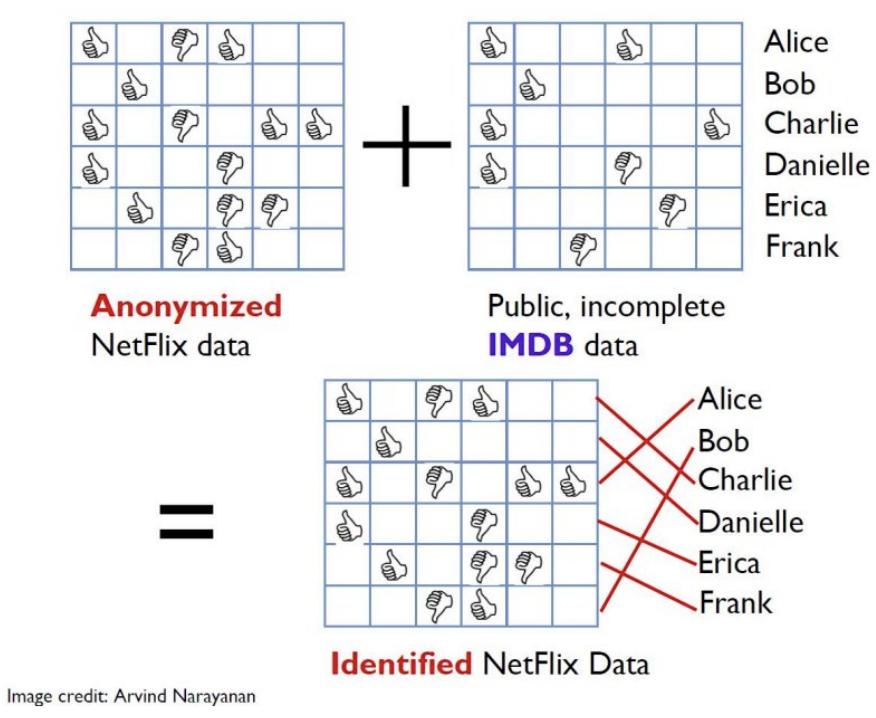
\includegraphics[width=0.6\linewidth]{Introduction/netflix.png}
	\caption{
	لطفا برای همه‌ی عکس‌ها کپشن بنویسید!
	}
\end{figure}


حال به مقاله‌ی دکتر ابراهیمی در مورد محرمانگی تفاضلی در گراف‌ها \cite{b1} ارجاع می‌زنم تا این راه هم دیده باشید:)